\documentclass[border=0.2cm]{standalone}

%\renewcommand{\raggedsection}{\centering}
\usepackage{sectsty}
\usepackage{lipsum}
\usepackage{cases}
\usepackage{tikz}
\usetikzlibrary{shapes.geometric}
\usetikzlibrary{calc}
\usetikzlibrary{arrows}
\usetikzlibrary{decorations.pathreplacing}

\begin{document}
	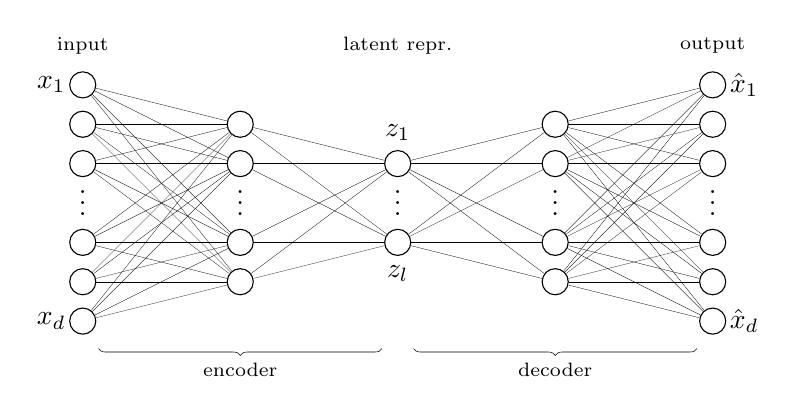
\begin{tikzpicture}
		\node (in) at (-4, 2) {\scriptsize input};

		\node (x1) at (-4.4, 1.5) {$x_1$};
		\node[circle,draw] (x11) at (-4, 1.5) {};
		\node[circle,draw] (x12) at (-4, 1) {};
		\node[circle,draw] (x13) at (-4, 0.5) {};
		\node (dots11) at (-4, 0.1) {$\vdots$};
		\node[circle,draw] (x14) at (-4, -0.5) {};
		\node[circle,draw] (x15) at (-4, -1) {};
		\node (xd) at (-4.4, -1.5) {$x_d$};
		\node[circle,draw] (x16) at (-4, -1.5) {};

		\node[circle,draw] (x21) at (-2, 1) {};
		\node[circle,draw] (x22) at (-2, 0.5) {};
		\node (dots21) at (-2, 0.1) {$\vdots$};
		\node[circle,draw] (x23) at (-2, -0.5) {};
		\node[circle,draw] (x24) at (-2, -1) {};
		
		\node (latent) at (0, 2) {\scriptsize latent repr.};
		\node (z1) at (0, 0.9) {$z_1$};
		\node[circle,draw] (x31) at (0, 0.5) {};
		\node (dots31) at (0, 0.1) {$\vdots$};
		\node (zl) at (0, -0.9) {$z_l$};
		\node[circle,draw] (x32) at (0, -0.5) {};

		\node[circle,draw] (x41) at (2, 1) {};
		\node[circle,draw] (x42) at (2, 0.5) {};
		\node (dots41) at (2, 0.1) {$\vdots$};
		\node[circle,draw] (x43) at (2, -0.5) {};
		\node[circle,draw] (x44) at (2, -1) {};
		
		\node (out) at (4, 2) {\scriptsize output};
		\node (xh1) at (4.4, 1.5) {$\hat{x}_1$};
		\node[circle,draw] (x51) at (4, 1.5) {};
		\node[circle,draw] (x52) at (4, 1) {};
		\node[circle,draw] (x53) at (4, 0.5) {};
		\node (dots51) at (4, 0.1) {$\vdots$};
		\node[circle,draw] (x54) at (4, -0.5) {};
		\node[circle,draw] (x55) at (4, -1) {};
		\node (xhd) at (4.4, -1.5) {$\hat{x}_d$};
		\node[circle,draw] (x56) at (4, -1.5) {};
		
		% input to hidden
		\path [-, line width=0.1pt] (x11) edge (x21);
		\path [-, line width=0.1pt] (x11) edge (x22);
		\path [-, line width=0.1pt] (x11) edge (x23);
		\path [-, line width=0.1pt] (x11) edge (x24);

		\path [-, line width=0.1pt] (x12) edge (x21);
		\path [-, line width=0.1pt] (x12) edge (x22);
		\path [-, line width=0.1pt] (x12) edge (x23);
		\path [-, line width=0.1pt] (x12) edge (x24);

		\path [-, line width=0.1pt] (x13) edge (x21);
		\path [-, line width=0.1pt] (x13) edge (x22);
		\path [-, line width=0.1pt] (x13) edge (x23);
		\path [-, line width=0.1pt] (x13) edge (x24);

		\path [-, line width=0.1pt] (x14) edge (x21);
		\path [-, line width=0.1pt] (x14) edge (x22);
		\path [-, line width=0.1pt] (x14) edge (x23);
		\path [-, line width=0.1pt] (x14) edge (x24);

		\path [-, line width=0.1pt] (x15) edge (x21);
		\path [-, line width=0.1pt] (x15) edge (x22);
		\path [-, line width=0.1pt] (x15) edge (x23);
		\path [-, line width=0.1pt] (x15) edge (x24);

		\path [-, line width=0.1pt] (x16) edge (x21);
		\path [-, line width=0.1pt] (x16) edge (x22);
		\path [-, line width=0.1pt] (x16) edge (x23);
		\path [-, line width=0.1pt] (x16) edge (x24);
		
		% hidden to z
		\path [-, line width=0.1pt] (x21) edge (x31);
		\path [-, line width=0.1pt] (x21) edge (x32);

		\path [-, line width=0.1pt] (x22) edge (x31);
		\path [-, line width=0.1pt] (x22) edge (x32);

		\path [-, line width=0.1pt] (x23) edge (x31);
		\path [-, line width=0.1pt] (x23) edge (x32);

		\path [-, line width=0.1pt] (x24) edge (x31);
		\path [-, line width=0.1pt] (x24) edge (x32);

		% z to hidden layer
		\path [-, line width=0.1pt] (x31) edge (x41);
		\path [-, line width=0.1pt] (x31) edge (x42);
		\path [-, line width=0.1pt] (x31) edge (x43);
		\path [-, line width=0.1pt] (x31) edge (x44);

		\path [-, line width=0.1pt] (x32) edge (x41);
		\path [-, line width=0.1pt] (x32) edge (x42);
		\path [-, line width=0.1pt] (x32) edge (x43);
		\path [-, line width=0.1pt] (x32) edge (x44);
		
		% hidden to output
		\path [-, line width=0.1pt] (x41) edge (x51);
		\path [-, line width=0.1pt] (x41) edge (x52);
		\path [-, line width=0.1pt] (x41) edge (x53);
		\path [-, line width=0.1pt] (x41) edge (x54);
		\path [-, line width=0.1pt] (x41) edge (x55);
		\path [-, line width=0.1pt] (x41) edge (x56);

		\path [-, line width=0.1pt] (x42) edge (x51);
		\path [-, line width=0.1pt] (x42) edge (x52);
		\path [-, line width=0.1pt] (x42) edge (x53);
		\path [-, line width=0.1pt] (x42) edge (x54);
		\path [-, line width=0.1pt] (x42) edge (x55);
		\path [-, line width=0.1pt] (x42) edge (x56);

		\path [-, line width=0.1pt] (x43) edge (x51);
		\path [-, line width=0.1pt] (x43) edge (x52);
		\path [-, line width=0.1pt] (x43) edge (x53);
		\path [-, line width=0.1pt] (x43) edge (x54);
		\path [-, line width=0.1pt] (x43) edge (x55);
		\path [-, line width=0.1pt] (x43) edge (x56);

		\path [-, line width=0.1pt] (x44) edge (x51);
		\path [-, line width=0.1pt] (x44) edge (x52);
		\path [-, line width=0.1pt] (x44) edge (x53);
		\path [-, line width=0.1pt] (x44) edge (x54);
		\path [-, line width=0.1pt] (x44) edge (x55);
		\path [-, line width=0.1pt] (x44) edge (x56);
		
		\draw[decorate, decoration={brace}, yshift=1ex, line width=0.2pt]  (-0.2, -2) -- node[below=0.4ex] {\scriptsize encoder} (-3.8, -2);
		\draw[decorate, decoration={brace}, yshift=1ex, line width=0.2pt]  (3.8, -2) -- node[below=0.4ex] {\scriptsize decoder} (0.2, -2);

		
	\end{tikzpicture}

\end{document}
